\chapter{Results}\label{results}

In this chapter, we analyze two proposed idealized models of the TCPC. These models are designed to incorporate key geometric modifications identified as beneficial in reducing energy dissipation, as described in \cite{Rijnberg2018}. These modifications, summarized in Figure~\ref{fig:positive_modifications}, serve as a foundation for investigating the effects of caval offsetting, curving, flaring, and other geometric factors on flow dynamics.

\begin{figure}[H]
	\centering
	\includegraphics[width=0.65\textwidth]{figures/energyloss-en.pdf}
	\caption[Positive Modifications for TCPC]{Key modifications to improve TCPC geometry and reduce energy dissipation: (a) caval offsetting, where the inferior and superior vena cava are misaligned to minimize flow collision; (b) curving, where the conduits are curved to enhance flow alignment; (c) the Y-graft configuration, which splits the flow evenly between outlets; and (d) flaring, where the connections are widened to reduce sharp corners and flow resistance. Adapted from \cite{Rijnberg2018}.}
	\label{fig:positive_modifications}
\end{figure}

\section{The Models}

To systematically evaluate the effects of geometric changes, the models were developed with varying levels of complexity, incorporating different numbers of degrees of freedom. Both models represent idealized TCPC geometries and share the same labeling convention for inlets and outlets. Specifically, the inlets are denoted as $\Gamma^{N}_{\text{in}}$ (top inlet representing the superior vena cava) and $\Gamma^{S}_{\text{in}}$ (bottom inlet representing the inferior vena cava with the conduit). The outlets are labeled as $\Gamma^{W}_{\text{out}}$ (left outlet representing the left pulmonary artery) and $\Gamma^{E}_{\text{out}}$ (right outlet representing the right pulmonary artery). The shared geometric framework, along with labeled boundaries, is illustrated in Figure~\ref{fig:junction schema}.

\begin{figure}[H]
	\centering
	\begin{subfigure}{0.45\textwidth}
		\centering
		\includegraphics[width=0.75\textwidth, trim={0mm -13mm 0mm 0mm}]{figures/3dschema.pdf}
		\caption{3D schematic of the idealized TCPC junction.}
		\label{fig:schema 3d}
	\end{subfigure}\hspace{2mm}
	\begin{subfigure}{0.53\textwidth}
		\centering
		\includegraphics[width=0.99\textwidth, trim={0mm -5mm 0mm 0mm}]{figures/2dschema.pdf}
		\caption{2D schematic of the idealized TCPC junction, highlighting labeled boundaries.}
		\label{fig:schema 2d}
	\end{subfigure}
	\vspace{2mm}
	\caption[Schematic of Idealized TCPC Geometry]{2D and 3D schematic illustrations of the idealized TCPC geometry, showing labeled inlets ($\Gamma^{N}_{\text{in}}$, $\Gamma^{S}_{\text{in}}$) and outlets ($\Gamma^{W}_{\text{out}}$, $\Gamma^{E}_{\text{out}}$).}
	\label{fig:junction schema}
\end{figure}


\subsection{Model 1: Simplified Cylindrical Junction}

The first model represents a basic cylindrical junction, where the bottom vertical cylinder corresponds to the inferior vena cava (IVC), the horizontal cylinder corresponds to the pulmonary artery, and the top vertical cylinder represents the superior vena cava (SVC). The IVC and SVC are connected perpendicularly to the pulmonary artery, creating a cross-like structure. 

Model 1 was chosen because it introduces only one degree of freedom: the vertical offset of the IVC relative to the SVC. This simplicity makes it feasible to sample and evaluate the optimization space exhaustively, providing an opportunity to study the behavior of the objective functions, namely wall shear stress (WSS) and turbulence kinetic energy (TKE), in detail.

\begin{figure}[H]
	\centering
	\includegraphics[width=0.8\textwidth]{figures/krizovatka-obecna.pdf} % Replace with your figure for Model 1
	\caption[Simplified Cylindrical Junction]{Schematic of Model 1: A simplified cylindrical junction with one degree of freedom, the vertical offset of the IVC relative to the SVC.}
	\label{fig:model1_schematic}
\end{figure}

\subsection{Model 2: Complex Geometric Model}

The second model introduces additional complexity by incorporating five degrees of freedom: the vertical offset of the IVC, the angles of connection for both the IVC and SVC to the pulmonary artery, the flaring of the IVC, and the width of the IVC. This model enables a more detailed investigation of the interaction between geometric parameters and hemodynamic efficiency.

Model 2 was selected because its higher complexity allows for greater variations in geometry and, consequently, a potentially larger impact on flow dynamics. However, the increased number of degrees of freedom makes it infeasible to sample the optimization space comprehensively, rendering the model more akin to a "black box" during optimization.

\begin{figure}[H]
	\centering
	\includegraphics[width=0.8\textwidth]{figures/krizovatka-obecna.pdf} % Replace with your figure for Model 2
	\caption[Complex Geometric Model]{Schematic of Model 2: A more complex model with five degrees of freedom—IVC offset, connection angles, flaring, and width of the IVC.}
	\label{fig:model2_schematic}
\end{figure}

\section{Objective functions and other monitored quantities}\label{objective funcs meaning}
Selecting appropriate objective functions is essential for guiding geometric optimization. In this work, we focus primarily on two such functions: the turbulence kinetic energy (TKE) and the shear rate near the walls. In addition, we also present other relevant metrics that are monitored during the computations.

\subsubsection*{Turbulence kinetic energy}
TKE, defined by~\eqref{eq:turb kin energy}, measures the intensity of velocity fluctuations within the flow. In the context of the TCPC, higher TKE generally corresponds to increased energy losses. Thus, reducing TKE in the TCPC region is desirable in order to improve hemodynamic efficiency. We sum TKE over a defined control volume within the computational domain, obtaining a global level of turbulent activity in the region. In the case of TCPC, TKE can serve as surrogate measure of how smoothly and efficiently blood flows through the connection. 

\subsubsection*{Shear rate}
Shear rate, defined in \eqref{eq:dot gamma}, provides insight into the mechanical forces acting on the vessel walls. Excessive shear rate can negatively affect the vascular health, making controlling near-wall shear rates crucial for ensuring the long-term patency and physiological compatibility of the TCPC.

However, measuring shear rate directly at the wall in a computational framework -- especially using LBM -- poses a challenge. The discrete nature of the grid and the no-slip boundary condition mean that the resolution near the wall can affect the computed shear rate and make it sensitive to discretization details. To address this, we introduce a thin layer of thickness 1 mm adjacent to the vessel walls. Within this layer, we sum the shear rate values rather than relying solely on the cells immediately neighboring the walls. This approach was chosen to reduce the sensitivity on grid characteristics while maintaining the physiological relevance of the quantity, ensuring it provides representative measure of local flow behavior. We denote this near-wall shear rate as $\dot{\gamma}^{A}_{\mathrm{nw}}$.

\subsubsection*{IVC and SVC flow split}
In addition to the main objective functions, we monitor how fluid from the inferior vena cava (IVC) and superior vena cava (SVC) divides between the left and right pulmonary arteries  (LPA and RPA, respectively). A balanced or at least minimally maintained split of inferior vena cava flow into both pulmonary artery branches is desirable. This metric is evaluated in post-processing using the computed mean velocity field. We denote the percentage of fluid directed to RPA as $F^{\text{RPA}}$ and to LPA as $F^{\text{LPA}}$, with subindices IVC and SVC used to specify the source of the flow.

\subsubsection*{Mean velocity vector angle at the pulmonary artery outlets}
It is beneficial for blood in the pulmonary arteries to flow downstream in a laminar manner. Thus, we examine the angle between the mean velocity vector and the outlet normal vector. This angle provides the information  for studying the laminarity of the flow.

\section{The models}

To systematically evaluate the effects of geometric changes, the models were developed with varying levels of complexity, incorporating different numbers of degrees of freedom. Both models represent idealized TCPC geometries and share the same labeling convention for inlets and outlets. 

The inlets are denoted as $\Gamma^{\text{N}}_{\text{in}}$ (representing the superior vena cava at the top) and $\Gamma^{\text{S}}_{\text{in}}$ (representing the inferior vena cava with the conduit at the bottom). Similarly, the outlets are labeled as $\Gamma^{\text{W}}_{\text{out}}$ (representing the left part of the pulmonary artery) and $\Gamma^{\text{E}}_{\text{out}}$ (representing the right part of the pulmonary artery).
The shared geometric framework and boundary labels, is illustrated in Figure~\ref{fig:junction schema}. The dimensions of cylindrical segments forming the simplified junction along with their corresponding abbreviations are presented in Table~\ref{tab:tcpc dims}.


\begin{figure}[H]
	\centering
	\vspace{2mm}
	\includegraphics[width=0.99\textwidth]{figures/3d-tcpc-schema-combined.pdf}
	\vspace{7mm}
	\caption{Schematic representation of the idealized TCPC geometry. The labeled inlets ($\Gamma^{\text{N}}_{\text{in}}$, $\Gamma^{\text{S}}_{\text{in}}$) and outlets ($\Gamma^{\text{W}}_{\text{out}}$, $\Gamma^{\text{E}}_{\text{out}}$), directions of inflows and outflows, and the dimensions of the cylindrical segments forming the junction are illustrated.}
	\label{fig:junction schema}
\end{figure}

\bgroup
\centering
\vspace{4mm}
\setlength\tabcolsep{3mm}
\def\arraystretch{1.7}%
\begin{tabular}{|l|l|c|c|}
	\hline
	Segment & Abbreviation & Length & Diameter \\ \hline
	Inferior vena cava 	& IVC 	&      39 mm        &     14 mm    \\ 
	Superior vena cava  & SVC 	&      39 mm     	&     14 mm     \\ 
	Pulmonary artery 	& PA 	&      170 mm     	&     22 mm     \\  \hline
\end{tabular}
\vspace{2mm}
\captionof{table}{Dimensions and abbreviations of the cylindrical segments forming the idealized TCPC junction.}
\vspace{4mm}
\label{tab:tcpc dims}
\egroup

In both models, the objective functions are studied within a defined control volume, denoted as A, which is a subset of the entire computational domain. By restricting the analysis to this region, we aim reduce potential errors introduced by the numerical boundary conditions. The control volume involves inlet and outlet boundaries named according to their respective vessel segments: \(\Gamma^{\text{SVC}}_{\text{in}}\) for the superior vena cava inlet, \(\Gamma^{\text{IVC}}_{\text{in}}\) for the inferior vena cava inlet, \(\Gamma^{\text{LPA}}_{\text{out}}\) for the left pulmonary artery outlet, and \(\Gamma^{\text{RPA}}_{\text{out}}\) for the right pulmonary artery outlet. The turbulence kinetic energy is evaluated in the entire control volume. The near-wall shear rate is examined along the boundaries of the control volume that are shared with the vessel walls.

\subsection*{Model 1: Simplified cylindrical junction}\label{mod:model1}
The first model represents a basic cylindrical junction where the IVC and SVC are connected perpendicularly to the PA, forming a cross-like structure, as illustrated in Figure~\ref{fig:model1_schematic}. Model 1 was chosen because it introduces only one degree of freedom, the horizontal offset of the IVC axis relative to the SVC, denoted by $o_1$. This simplicity makes it possible to sample the optimization space and evaluate the objective functions at the points of the sampling. This provides an opportunity to examine the behavior of the objective functions and verify the result generated by the optimization framework.

\subsection*{Model 2: More complex geometric model}\label{mod:model2}
Illustration of Model 2 is presented in Figure~\ref{fig:model1_schematic}. The second model introduces additional complexity by incorporating five degrees of freedom:
\begin{itemize}
	\item horizontal offset of the IVC axis, denoted by $o_1$,
	\item angle of the IVC axis, denoted by $\alpha_1$,
	\item angle of the SVC axis, denoted by $\alpha_2$,
	\item width and curvature of the IVC-PA connection, denoted by $f_1$,
	\item width and curvature of the SVC-PA connection, denoted by $f_2$.
%	\item width of the IVC, denoted by $l_1$.
\end{itemize}
Model 2 was selected because its higher complexity allows for more geometric variations.

\begin{figure}[H]
	\begin{subfigure}{0.48\textwidth}
		\centering
		\includegraphics[width=0.91\textwidth, trim={0 0 0 0}]{figures/model1.pdf}
		\caption[Simplified Cylindrical Junction]{Schematic of Model 1: A simplified cylindrical junction with one degree of freedom, the horizontal offset of the IVC.}
		\label{fig:model1_schematic}
	\end{subfigure}\hfill%
	\begin{subfigure}{0.48\textwidth}
		\centering
		\includegraphics[width=0.91\textwidth]{figures/model2.pdf}
		\caption[Complex Geometric Model]{Schematic of Model 2: A more complex model introducing five degrees of freedom: IVC offset, connection angles and flaring.}
		\label{fig:model2_schematic}
	\end{subfigure}
	\vspace{4mm}
	\caption{Schematic illustrations of Model 1 and Model 2.}
	\label{fig:model schemas}
\end{figure}
\section{Problem with one optimization parameter}

\subsection{Problem setup}
\begin{problem}{Basic cylindrical junction}
	\vspace{2mm}
	Physical setup:
	\begin{itemize}
		\item Domain: $ \Omega=(0 ; 170 \mathrm{~mm}) \times(0 ; 22 \mathrm{~mm}) \times(0 ; 100 \mathrm{~mm})$.
		\item Kinematic viscosity: $ \nu=3 \cdot 10^{-6} \mathrm{~m}^{2} \mathrm{~s}^{-1}$.
		\item Inflow at $\Gamma^{\text{IVC}}_{\text{in}}$: a constant velocity of magnitude $0{,}45$ \si{m s^{-1}},  aligned with the IVC axis in the positive $x_3$-direction.
		\item Inflow at $\Gamma^{\text{SVC}}_{\text{in}}$: a constant velocity of magnitude $0{,}35$ \si{m s^{-1}}, aligned with the SVC axis in the negative $x_3$-direction.
	\end{itemize} 
	LBM setup:
	\begin{itemize}
		\item Initial condition on $ \overline{\hat{\Omega}} $ set as described in Section~\ref{pocatecni podminka}.
		\item Boundary conditions at $\Gamma^{\text{W}}_{\text{out}}$ and $\Gamma^{\text{E}}_{\text{out}}$ set according to Section~\ref{symmetric bc}.
		\item Discretization: $\overline{\hat{\Omega}} = N_{x} \times N_{y} \times N_{z}$, $N_{x} = 768, \, N_{y} = 105, N_{z} = 453$.
		\item Kinematic viscosity in lattice units: $\nu^{L} = 10^{-3} $.
	\end{itemize}
	Optimzation setup:
	\begin{itemize}
		\item Using Model 1, as described in Section~\ref{mod:model1} and illustrated in Figure~\ref{fig:model1_schematic}.
		\item Using the custom Nelder–Mead and MADS (NOMAD implementation) methods, both described in Chapter~\ref{optimization}
	\end{itemize}
	\label{prob:1}
\end{problem}
\newpage
\subsection{Results and discussion}


\begin{figure}[H]
	\subsubsection*{Mean velocities}
	{\centering
	\begin{subfigure}{0.48\textwidth}
		\centering
		\includegraphics[
			width=\textwidth,
			trim={0mm 0mm 0mm 0mm}
		]
			{figures/plots/08/08_mean_veloc_XZ-c.pdf}
	\end{subfigure}\hfill%
	\begin{subfigure}{0.48\textwidth}
		\centering
		\includegraphics[
		width=\textwidth,
		trim={0mm 0mm 0mm 0mm}
		]
		{figures/plots/08/08_mean_veloc_XZ-c.pdf}
	\end{subfigure}
	\begin{center}
			\includegraphics[
		width=0.4\textwidth,
		trim={0mm 0mm 0mm 0mm}
		]
		{figures/plots/08/veloc_legend.pdf}
	\end{center}
	}

%	\begin{subfigure}{0.24\textwidth}
%		\centering
%		\includegraphics[
%		width=0.8\textwidth,
%		trim={0mm 0mm 0mm 0mm}
%		]
%		{figures/plots/08/08_LPA_veloc-c.pdf}
%		\caption{}
%	\end{subfigure}\hfill%
%	\begin{subfigure}{0.24\textwidth}
%		\centering
%		\includegraphics[
%		width=0.8\textwidth,
%		trim={0mm 0mm 0mm 0mm}
%		]
%		{figures/plots/08/08_RPA_veloc-c.pdf}
%		\caption{}
%	\end{subfigure}
%	\begin{subfigure}{0.24\textwidth}
%		\centering
%		\includegraphics[
%		width=0.8\textwidth,
%		trim={0mm 0mm 0mm 0mm}
%		]
%		{figures/plots/08/08_LPA_angle-c.pdf}
%		\caption{}
%	\end{subfigure}
%	\begin{subfigure}{0.24\textwidth}
%		\centering
%		\includegraphics[
%		width=0.8\textwidth,
%		trim={0mm 0mm 0mm 0mm}
%		]
%		{figures/plots/08/08_RPA_angle-c.pdf}
%		\caption{}
%	\end{subfigure}
%	}
%	\subsubsection*{Model 1: Simplified cylindrical junction}
%	\begin{subfigure}{1.0\textwidth}
%		\centering
%		\includegraphics[
%		width=1.0\textwidth,
%		trim={60mm 10mm 60mm 0mm}
%		]
%		{figures/plots/08/08_mean_flucs_3D.pdf}
%		\caption{}
%	\end{subfigure}\hfill%
	\vspace{2mm}
	\caption{}
	\label{fig:}

\end{figure}


\section{Problem with multiple optimization parameters}\label{optim2}

\section{Results summary}

\todo[inline]{TBA. Recap of what was calculated. Mention that the feasibility of the proposed framework was showed. It can answer complex questions. Improving the optim process for the future to work more globally, that is possible thanks to modularity. Mention that the results suggest not only tht the framework works but that LBM thanks to its nature can be effectively used for extensive qualitative analysis of cardiovascular system providing valuable insight.}